\documentclass[11pt,a4paper]{article}

\usepackage[T1]{fontenc}
\usepackage[utf8]{inputenc}
\usepackage{lmodern}
\usepackage[margin=2.5cm]{geometry}
\usepackage{xcolor}
\usepackage{listings}
\usepackage{booktabs}
\usepackage{tabularx}
\usepackage{enumitem}
\usepackage{tikz}
\usetikzlibrary{positioning,arrows.meta}
\usepackage[hidelinks]{hyperref}

\definecolor{codebg}{gray}{0.95}
\lstset{
  language=bash,
  basicstyle=\ttfamily\small,
  backgroundcolor=\color{codebg},
  frame=single,
  rulecolor=\color{gray!50},
  breaklines=true,
  columns=fullflexible,
  keepspaces=true,
  showstringspaces=false,
  upquote=true,
  literate={~}{{\textasciitilde}}1,
}
\newcommand{\cmd}[1]{\texttt{#1}}

\title{How the \texttt{devtools} script works}
\date{}

\begin{document}
\maketitle

\begin{abstract}
\noindent \cmd{devtools} is a single Bash script that sets up and keeps up to date a
set of development tools on any Ubuntu machine. It is \emph{idempotent}: every step
first checks what is already there and only installs or upgrades what is missing or
out of date, so running it again is safe. This document describes the generic
machinery of the script: how it is organised, how steps are declared and run, the
shared helpers, and how command-line options change what runs. It deliberately does
not list the individual tools; those live in the arrays at the top of the script.
\end{abstract}

\tableofcontents

\section{Running it}

On a fresh machine the script is piped straight from GitHub into Bash:

\begin{lstlisting}
curl -fsSL https://raw.githubusercontent.com/andimon/devtools/main/devtools | bash
\end{lstlisting}

\noindent From a checkout it can be run directly, with options:

\begin{lstlisting}
./devtools                 # everything
./devtools --no-<step>     # everything except <step>
./devtools <tool> ...      # only the build deps and the named asdf tools
./devtools --help
\end{lstlisting}

\section{Overall flow}

The script runs top to bottom in one pass. Figure~\ref{fig:flow} shows the order.

\begin{figure}[h]
\centering
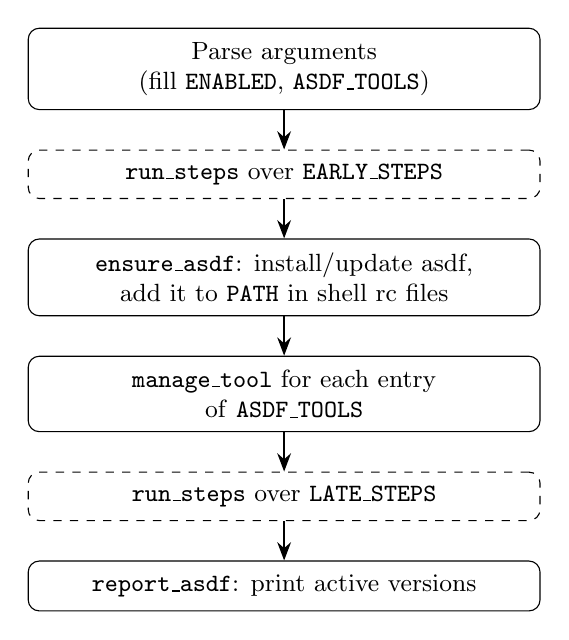
\begin{tikzpicture}[
  node distance=5mm,
  box/.style={draw, rounded corners, align=center, minimum width=6.5cm, inner sep=5pt, font=\small},
  opt/.style={box, dashed},
  arrow/.style={-{Stealth}, thick}
]
\node[box] (args) {Parse arguments\\(fill \cmd{ENABLED}, \cmd{ASDF\_TOOLS})};
\node[opt, below=of args] (early) {\cmd{run\_steps} over \cmd{EARLY\_STEPS}};
\node[box, below=of early] (asdf) {\cmd{ensure\_asdf}: install/update asdf,\\add it to \cmd{PATH} in shell rc files};
\node[box, below=of asdf] (tools) {\cmd{manage\_tool} for each entry\\of \cmd{ASDF\_TOOLS}};
\node[opt, below=of tools] (late) {\cmd{run\_steps} over \cmd{LATE\_STEPS}};
\node[box, below=of late] (report) {\cmd{report\_asdf}: print active versions};
\foreach \a/\b in {args/early, early/asdf, asdf/tools, tools/late, late/report}
  \draw[arrow] (\a) -- (\b);
\end{tikzpicture}
\caption{Order of execution. Dashed boxes are optional steps that can be switched off.}
\label{fig:flow}
\end{figure}

\noindent The script starts with \cmd{set -euo pipefail}: it stops at the first
command that fails, treats unset variables as errors, and makes a pipeline fail
if any command in it fails. Steps that are allowed to fail without stopping the
run (for example updating a plugin) say so explicitly with \cmd{|| warn \ldots}.

\section{Configuration at the top}

Everything that changes from time to time is kept in arrays at the top of the
script, so adding a tool rarely means touching the logic:

\begin{center}
\begin{tabularx}{\linewidth}{@{}lX@{}}
\toprule
Variable & Meaning \\
\midrule
\cmd{ASDF\_TOOLS} & Language runtimes installed through asdf, in order. A tool whose version depends on another must come after it. \\
\cmd{ALL\_TOOLS} & A copy of the full list, used to validate arguments and keep the order when filtering. \\
\textit{data arrays} & Lists consumed by individual steps (for example package names or application ids). \\
\cmd{EARLY\_STEPS} & Optional steps that run before asdf. \\
\cmd{LATE\_STEPS} & Optional steps that run after the asdf tools. \\
\cmd{STEPS} & Both lists joined; it drives \cmd{-{}-help} and the \cmd{-{}-no-}\textit{step} flags. \\
\cmd{ENABLED} & Associative array, step name $\to$ 1 (run) or 0 (skip). Every step starts at 1. \\
\bottomrule
\end{tabularx}
\end{center}

\noindent Each step name maps to a function by a fixed rule: \cmd{setup\_} followed by the
name with dashes turned into underscores, so \cmd{my-step} runs \cmd{setup\_my\_step}.
Adding a new optional step therefore takes two changes: write \cmd{setup\_}\textit{name}
and add \textit{name} to \cmd{EARLY\_STEPS} or \cmd{LATE\_STEPS}. The help text and the
\cmd{-{}-no-}\textit{name} flag come for free.

\section{Command-line options}

Each argument is handled in one \cmd{case} statement:

\begin{description}[style=nextline]
\item[\cmd{-{}-no-}\textit{step}] Sets \cmd{ENABLED[}\textit{step}\cmd{]=0}. An unknown step
  (or an empty one, \cmd{-{}-no-}) is rejected with \cmd{unknown argument}.
\item[\cmd{-h}, \cmd{-{}-help}] Prints the usage line, built from \cmd{STEPS}, and exits.
\item[\textit{tool}] Any other word must be one of \cmd{ALL\_TOOLS}; it is added to \cmd{SELECTED}.
\end{description}

\noindent When at least one tool is named, the run is narrowed down:

\begin{itemize}
\item \cmd{ASDF\_TOOLS} is rebuilt by walking \cmd{ALL\_TOOLS} and keeping only the
  selected ones. Walking the full list, rather than copying \cmd{SELECTED}, keeps the
  fixed order whatever order the tools were typed in.
\item Every step except \cmd{system} is switched off, because the build dependencies
  are needed to compile the runtimes.
\end{itemize}

\section{Helper functions}

Small helpers keep the step functions short and remove repeated code.

\begin{center}
\begin{tabularx}{\linewidth}{@{}lX@{}}
\toprule
Helper & What it does \\
\midrule
\cmd{log}, \cmd{warn}, \cmd{die} & Print a coloured message; \cmd{warn} and \cmd{die} write to stderr and \cmd{die} exits with status 1. \\
\cmd{have} \textit{cmd} & True if \textit{cmd} is on \cmd{PATH}. \\
\cmd{contains} \textit{x list\ldots} & True if \textit{x} is one of the list items. \\
\cmd{as\_root} \textit{cmd\ldots} & Runs the command directly when already root, otherwise through \cmd{sudo}. \\
\cmd{need\_apt} \textit{msg} & Warns and fails when \cmd{apt-get} is missing; used as \cmd{need\_apt "\ldots" || return}. \\
\cmd{apt\_update} & \cmd{apt-get update -qq} as root. \\
\cmd{apt\_install\_or\_upgrade} & Installs a package, or runs \cmd{-{}-only-upgrade} if \cmd{dpkg} already knows it. \\
\cmd{ensure\_apt\_repo} & Adds a vendor's signing key and a deb822 \cmd{.sources} file (read from stdin), unless a \cmd{.sources} or \cmd{.list} file with that name already exists, then refreshes apt. \\
\cmd{run\_remote\_script} & Downloads a script to a temporary file, runs it with the given interpreter, then deletes it. \\
\cmd{run\_steps} \textit{steps\ldots} & For each step that is enabled, calls its \cmd{setup\_} function. \\
\bottomrule
\end{tabularx}
\end{center}

\section{Step patterns}

Every optional step is a \cmd{setup\_}\textit{name} function. Most follow one of a few
patterns built from the helpers above.

\subsection{Plain apt package}
Call \cmd{need\_apt}, then \cmd{apt\_install\_or\_upgrade} for each package, often
looping over a data array declared at the top of the script.

\subsection{Vendor apt repository}
Register the vendor's repository with \cmd{ensure\_apt\_repo}, then install the
package with \cmd{apt\_install\_or\_upgrade}:

\begin{lstlisting}
setup_example() {
    need_apt "install example manually" || return
    local keyring=/etc/apt/keyrings/example.gpg
    ensure_apt_repo example Vendor example \
        https://vendor.example/key.gpg "$keyring" cat <<EOF
Types: deb
URIs: https://vendor.example/packages
Suites: stable
Components: main
Signed-By: $keyring
EOF
    apt_install_or_upgrade example example
}
\end{lstlisting}

\noindent The last argument of \cmd{ensure\_apt\_repo} is a filter for the downloaded key:
\cmd{gpg -{}-dearmor} turns an ASCII-armoured key into binary form, while \cmd{cat}
stores the key as it comes. Because the existence check also accepts a \cmd{.list}
file, a repository that was added by hand following the vendor's own instructions
is reused rather than added twice.

\subsection{Official installer script}
When a tool ships its own installer and updater, the step checks whether the tool
is present and was installed by that installer. If so it runs the tool's own update
command; if it was installed some other way it is left alone; otherwise the installer
is fetched and run with \cmd{run\_remote\_script}.

\subsection{Other package managers}
Steps that use another package manager (for example a sandboxed app store) first
make sure the manager and its remote exist, then install or update every id from
the corresponding data array.

\section{asdf (always runs)}
\cmd{ensure\_asdf} puts \cmd{\textasciitilde/.local/bin} and the asdf shims on \cmd{PATH} for the rest
of the run, then finds the newest asdf release by following GitHub's
\cmd{/releases/latest} redirect. It compares that tag with \cmd{asdf -{}-version}:

\begin{itemize}
\item same version: nothing to do;
\item an asdf exists somewhere other than \cmd{\textasciitilde/.local/bin}: warn and leave it alone;
\item otherwise: download the release archive for the machine's architecture
  (amd64 or arm64) and install the binary into \cmd{\textasciitilde/.local/bin}.
\end{itemize}

\noindent It then calls \cmd{setup\_shell\_rc}, which appends a block between the markers
\cmd{\# >>> devtools asdf >>>} and \cmd{\# <<< devtools asdf <<<} to \cmd{\textasciitilde/.bashrc} and,
if zsh is installed, \cmd{\textasciitilde/.zshrc}. The marker check means the block is added only once.

\section{Managed runtimes}
\cmd{manage\_tool} runs for each entry of \cmd{ASDF\_TOOLS}:

\begin{enumerate}
\item Add the asdf plugin, or update it if present.
\item Work out the newest version with \cmd{latest\_version}. By default this is
  \cmd{asdf latest}; a tool gets its own \cmd{case} branch only when that picks the
  wrong version (for example to skip pre-releases, or to stay compatible with a
  runtime installed earlier in the same run).
\item Install that version if it is not already installed.
\item Make it the user's default (\cmd{asdf set -{}-home}, or \cmd{asdf global} on old asdf)
  and refresh the shims.
\end{enumerate}

\section{Final report}
\cmd{report\_asdf} prints the version that \cmd{asdf current} reports for each tool that was
managed in this run, then the script prints \emph{Done.}

\section{Continuous integration}
The GitHub Actions workflow in \cmd{.github/workflows/test.yml} has two jobs:

\begin{description}
\item[lint] runs \cmd{shellcheck} and checks that \cmd{-{}-help} works and that bad arguments
  are rejected.
\item[install] runs the script twice on a clean Ubuntu runner and after each run
  checks that every tool is installed and that this document builds with
  \cmd{latexmk}. The second run proves that re-running is safe. The workflow also
  runs weekly to catch upstream changes such as moved download URLs or rotated
  signing keys.
\end{description}

\noindent To build this document locally:

\begin{lstlisting}
latexmk -pdf docs/devtools.tex
\end{lstlisting}

\section{Extending the script}
\begin{itemize}
\item \textbf{Another asdf runtime}: add it to \cmd{ASDF\_TOOLS}; add a case to
  \cmd{latest\_version} only if \cmd{asdf latest} picks the wrong version.
\item \textbf{Another item for an existing step}: add it to that step's data array.
\item \textbf{A new optional step}: write a \cmd{setup\_}\textit{name} function using one
  of the patterns above and add \textit{name} to \cmd{EARLY\_STEPS} or \cmd{LATE\_STEPS}.
\item \textbf{Always} add a check for it to the CI verify list.
\end{itemize}

\noindent Changes like these do not require updating this document. Changes to the
generic machinery (flow, argument handling, helpers, step patterns, asdf handling,
CI structure) do.

\end{document}
